\begin{frame}[t]{Conclusão}
    \transboxout[duration=0.5]
    \framesubtitle{Inovações} 

O dispositivo apresentou a capacidade:
\begin{itemize}
    \item Manipular informações e armazená-las permanentemente
    \item Bits definindo propriedades mecânicas
    \item O estado dos bits poder ser controlados remotamente por campos magnéticos 
\end{itemize}
\only<2->{
    \begin{alertblock}{}
        Nunca antes um dispositivo demonstrou ter estas duas propriedades simultâneamente.
    \end{alertblock}

}
 %*----------- notes
    \note[item]{Notes can help you to remember important information. Turn on the notes option.}
\end{frame}



\begin{frame}[t]{Conclusão}
    \transboxout[duration=0.5]
    \framesubtitle{Limitações} 
    \begin{itemize}
        \item Geometria complexa
        \item Complexidade na fabricação
        \item Densidade de armazenamento
    \end{itemize}
    \begin{figure}
        \begin{figure}[H]
            \centering
            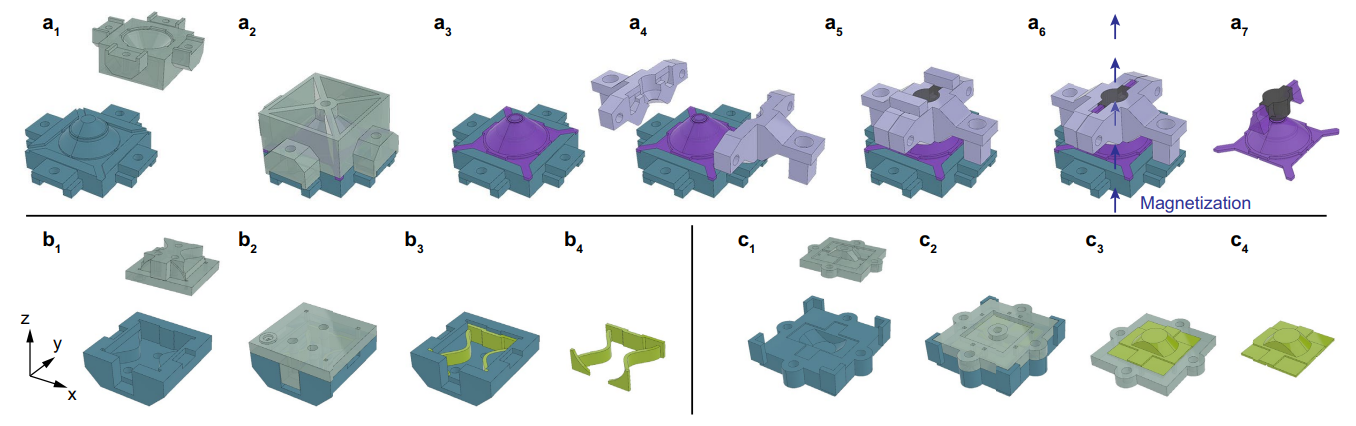
\includegraphics[width = 0.7\textwidth]{source/pictures/fabrication.png}
            \caption{Processo de fabricação\cite{chen2021reprogrammable}.}
            \label{fig:uba-fabrication}
        \end{figure}
        %\caption{.}
    \end{figure}
    \small
\end{frame}


\begin{frame}{Conclusão}
    \framesubtitle{Aplicações}
    
    \centering % Para centralizarmos o vídeo
    \includemedia[
    label=nome_qualquer, % ! Importante para linkar o vídeo ao botão (ver abaixo)
    width=0.6\linewidth, height=0.375\linewidth, % Dimensões
    addresource=./source/movies/compress-material.mp4, % ESTE É O SEU ARQUIVO DE VÍDEO (mesmo dir.)
    transparent, % Opções para que o player tenha transparência
    activate=pageopen, % Se você deseja que o vídeo esteja "carregado" ao abrir a página
    flashvars={
    source=./source/movies/compress-material.mp4
    &loop=true % Se você quer que o vídeo repita automaticamente 
    &scaleMode=letterbox % Manter proporções (dimensionais) do vídeo
    }
    ]{}{VPlayer.swf}
    \vspace{1cm} % Espaçamento entre vídeo e botão
    
    % Agora, você cria o botão para dar play/pause. Neste caso, o botão é apenas a letra "pi".
    
    \mediabutton[
    mediacommand=nome_qualquer:playPause,
    overface=\color{black}{{\strut $\pi$}},
    downface=\color{gray}{{\strut $\pi$}}
    ]{{\strut $\pi$}}
    
    
\end{frame}
